%% ═══════════════════════════════════════════════════════════════════════════
%%  Hybrid Semantic Prototype Weighting and Learning-to-Rank
%%  for Automated Bug Assignment
%%  — Full Research Paper (combined from peper.tex + pipeline_schema.tex) —
%% ═══════════════════════════════════════════════════════════════════════════
\documentclass[10pt,conference]{IEEEtran}

% ── Packages ──────────────────────────────────────────────────────────────────
\usepackage[T1]{fontenc}
\usepackage[utf8]{inputenc}
\usepackage{amsmath,amssymb}
\usepackage{algorithm}
\usepackage{algpseudocode}
\usepackage{booktabs}
\usepackage{array}
\usepackage{hyperref}
\usepackage{microtype}
\usepackage{cite}
\usepackage{graphicx}
\usepackage{xcolor}
\usepackage{tikz}
\usepackage{mdframed}
\usepackage{caption}
\usepackage{float}

% ── TikZ libraries ────────────────────────────────────────────────────────────
\usetikzlibrary{
  shapes.geometric, shapes.misc,
  arrows.meta, fit,
  positioning, backgrounds,
  calc, shadows.blur
}

% ── Color Palette (restrained academic) ───────────────────────────────────────
\definecolor{navydark}   {HTML}{1B2A4A}
\definecolor{navymid}    {HTML}{2E4A7A}
\definecolor{tealaccent} {HTML}{1A6B72}
\definecolor{slateblue}  {HTML}{3A4F8A}
\definecolor{indigomid}  {HTML}{4A3A8A}
\definecolor{mulberry}   {HTML}{6B2E5A}
\definecolor{crimsonmid} {HTML}{7A2A2A}
\definecolor{forestmid}  {HTML}{1A5C3A}
\definecolor{guardbg}    {HTML}{4A4A4A}
\definecolor{darktext}   {HTML}{1A1A2E}
\definecolor{arrowcol}   {HTML}{5A6A8A}

% ── TikZ Global Styles ────────────────────────────────────────────────────────
\tikzset{
  iobox/.style={
    rectangle, rounded corners=5pt,
    minimum width=7.2cm, minimum height=1.05cm,
    text centered, font=\small\bfseries,
    draw=#1, fill=#1!10, text=#1!80!black, line width=1.2pt
  },
  stepbox/.style={
    rectangle, rounded corners=4pt,
    minimum width=7.2cm, minimum height=1.15cm,
    text centered, font=\small,
    draw=#1, fill=#1!7, text=darktext, line width=0.9pt
  },
  stepnum/.style={
    circle, minimum size=0.58cm,
    fill=#1, text=white,
    font=\bfseries\scriptsize, inner sep=0pt, line width=0pt
  },
  phasegroup/.style={
    rectangle, rounded corners=6pt,
    draw=#1!50, fill=#1!4,
    dashed, line width=0.8pt,
    inner xsep=12pt, inner ysep=8pt
  },
  myarrow/.style={-Stealth, line width=1.2pt, color=arrowcol},
  dasharrow/.style={-Stealth, line width=0.9pt, color=arrowcol, dashed},
  sidenode/.style={
    rectangle, rounded corners=3pt,
    minimum width=3.2cm, minimum height=0.75cm,
    text centered, font=\scriptsize,
    draw=#1!60, fill=#1!6, text=darktext, line width=0.7pt
  },
  guardrail/.style={
    rectangle, rounded corners=4pt,
    dashed, line width=0.8pt,
    minimum width=7.2cm, minimum height=1.0cm,
    text centered, font=\small\itshape,
    draw=guardbg!60, fill=guardbg!6, text=darktext
  }
}

% ── Hyperlink setup ───────────────────────────────────────────────────────────
\hypersetup{
  colorlinks=true,
  linkcolor=navymid,
  citecolor=navymid,
  urlcolor=navymid
}

% ── Algorithm style ───────────────────────────────────────────────────────────
\algrenewcommand\algorithmicrequire{\textbf{Input:}}
\algrenewcommand\algorithmicensure{\textbf{Output:}}
\algnewcommand{\LineComment}[1]{\State \(\triangleright\) \textit{#1}}

% ── mdframed step-box style ───────────────────────────────────────────────────
\newmdenv[
  linewidth=1.2pt, roundcorner=4pt,
  innertopmargin=7pt, innerbottommargin=7pt,
  innerleftmargin=10pt, innerrightmargin=10pt,
  skipabove=6pt, skipbelow=2pt
]{stepframe}

%% ════════════════════════════════════════════════════════════════════════════
\begin{document}

% ── Title & Author ────────────────────────────────────────────────────────────
\title{Hybrid Semantic Prototype Weighting and\\
       Learning-to-Rank for Automated Bug Assignment}

\author{
  \IEEEauthorblockN{Suyash Srivastava}
  \IEEEauthorblockA{Independent Researcher\\
  India\\
  \texttt{suyash1527@gmail.com}}
}
\maketitle

%% ════════════════════════════════════════════════════════════════════════════
%% ABSTRACT
%% ════════════════════════════════════════════════════════════════════════════
\begin{abstract}
Automated bug assignment aims to reduce triage time in software maintenance
by recommending the most suitable developers to fix newly reported bugs.
Traditional approaches rely on static keyword-based heuristics or simple
similarity metrics that fail to capture the nuanced semantic intent of a bug
report.
In this paper we propose a novel pipeline consisting of
\emph{Hybrid Semantic Prototype Weighting} paired with a
\emph{Learning-to-Rank} (LTR) model.
A Weighted Sum Model (WSM) first computes candidate scores using dynamic
weights derived from cosine similarities between the bug embedding and six
curated ``prototype sentences'' that represent ideal developer attributes.
An XGBoost Ranker then refines the candidate order using a 19-dimensional
feature vector --- spanning developer attributes, bug-developer interaction
features, severity flags, and semantic prototype scores --- together with
historical resolution data, and incorporating a confidence-based fallback
mechanism.
Evaluated on four open-source Bugzilla repositories (Eclipse IDE, Mozilla
Firefox, Mozilla Core, and Thunderbird), our LTR approach consistently
outperforms the semantic WSM baseline, achieving Top-1 accuracy of
\textbf{26.50\%} and MRR of \textbf{0.4239} on Eclipse (a \textbf{+4.50pp}
improvement), with similar gains across all four projects.
\end{abstract}

\begin{IEEEkeywords}
Bug Assignment, Machine Learning, Natural Language Processing,
Learning to Rank, Semantic Embeddings, XGBoost
\end{IEEEkeywords}

%% ════════════════════════════════════════════════════════════════════════════
%% I. INTRODUCTION
%% ════════════════════════════════════════════════════════════════════════════
\section{Introduction}

As software systems grow in complexity, bug-tracking repositories (e.g.,
Bugzilla, Jira) receive hundreds of bug reports daily.
Manual triage is a time-consuming and error-prone process.
The \emph{bug assignment problem} involves recommending a ranked list of
candidate developers who possess the right expertise, availability, and
historical context to resolve a given bug efficiently.

While existing approaches often use Term Frequency--Inverse Document
Frequency (TF-IDF)~\cite{salton1988tfidf} or topic modelling combined with classification
algorithms (such as SVM or Na\"{i}ve Bayes)~\cite{cubranic2004hipikat, anvik2006triage}, they commonly struggle with
vocabulary mismatch and synonyms.
Recent work has explored transformer-based embeddings to address these
limitations~\cite{zaidi2022transformers}, as well as ensemble learning
methods for rapid triage in IoT contexts~\cite{yin2018elm}.
Furthermore, traditional heuristics rely on hardcoded keyword lists to
assess aspects like ``urgency'' or ``experience required.''

In this work we introduce a hybrid framework that bridges modern semantic
Natural Language Processing (NLP) with Learning-to-Rank algorithms.
We replace brittle keyword lists with \emph{Semantic Prototype Weighting},
dynamically scoring bug reports against ``ideal'' natural language sentences
using dense transformer embeddings~\cite{reimers2019sentencetransformers}.
Finally, we train an XGBRanker~\cite{chen2016xgboost} to optimise the final
developer rankings using a pairwise learning-to-rank
objective~\cite{liu2009ltr}, ensuring high precision while maintaining
robust fallback behaviour.

%% ════════════════════════════════════════════════════════════════════════════
%% II. METHODOLOGY
%% ════════════════════════════════════════════════════════════════════════════
\section{Methodology}

%% ── II-A  Pipeline Overview ─────────────────────────────────────────────────
\subsection{Pipeline Overview}

Figure~\ref{fig:pipeline} illustrates the complete eight-step pipeline from
incoming bug report to final ranked developer list.
The three shaded regions denote the logical phases of the system:
\emph{Encoding}, \emph{Candidate Selection}, and \emph{Ranking}.

\begin{figure*}[t]
\centering
\resizebox{\textwidth}{!}{%
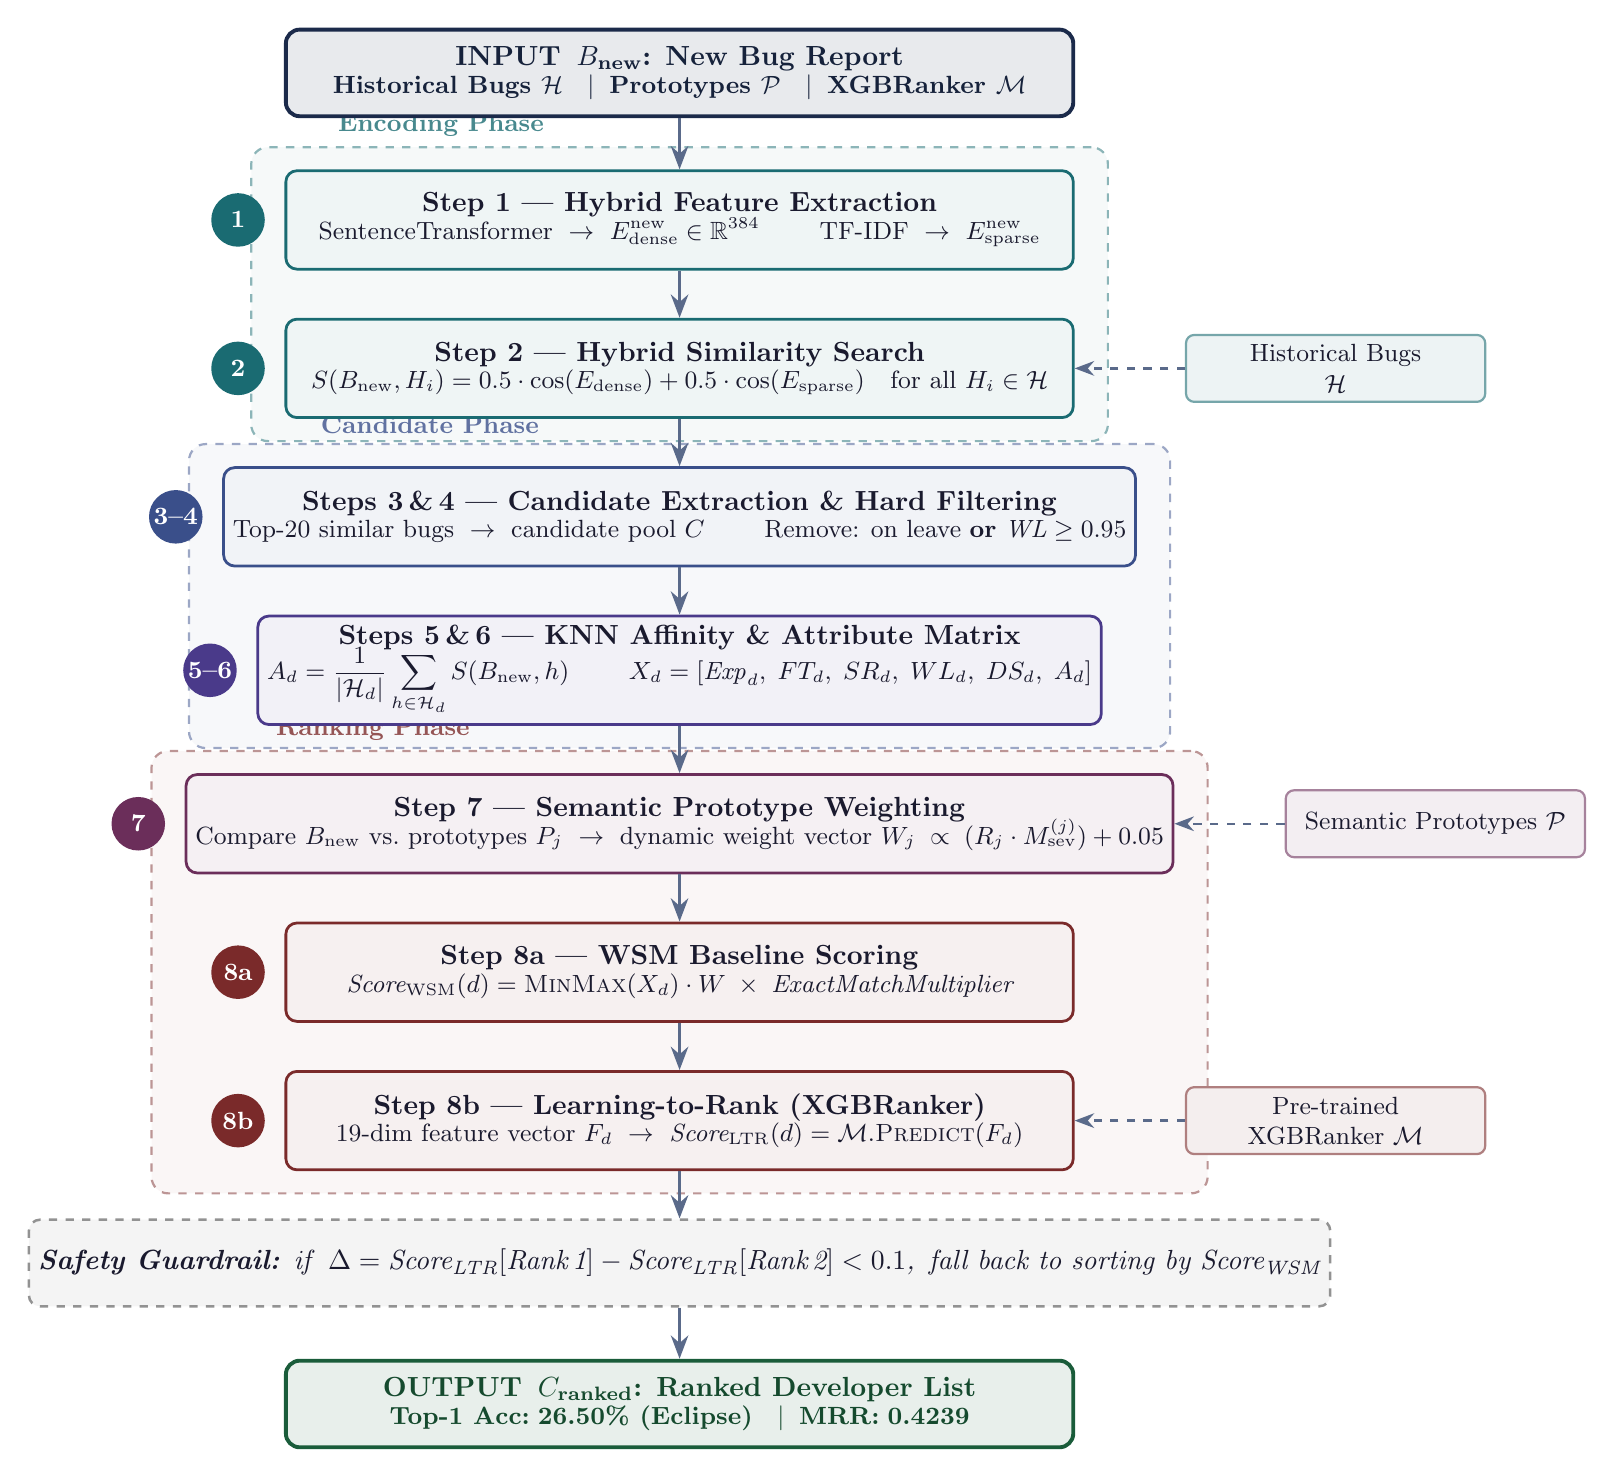
\begin{tikzpicture}[node distance=0.7cm,
                    every node/.style={align=center}]

  \tikzset{
    iobox/.style={
      rectangle, rounded corners=5pt,
      minimum width=10cm, minimum height=1.1cm,
      text centered, font=\normalsize\bfseries,
      draw=#1, fill=#1!10, text=#1!80!black, line width=1.4pt
    },
    stepbox/.style={
      rectangle, rounded corners=4pt,
      minimum width=10cm, minimum height=1.25cm,
      text centered, font=\normalsize,
      draw=#1, fill=#1!7, text=darktext, line width=1.0pt
    },
    guardrail/.style={
      rectangle, rounded corners=4pt, dashed, line width=0.9pt,
      minimum width=10cm, minimum height=1.1cm,
      text centered, font=\normalsize\itshape,
      draw=guardbg!60, fill=guardbg!6, text=darktext
    },
    sidenode/.style={
      rectangle, rounded corners=3pt,
      minimum width=3.8cm, minimum height=0.85cm,
      text centered, font=\small,
      draw=#1!60, fill=#1!8, text=darktext, line width=0.8pt
    },
    stepnum/.style={
      circle, minimum size=0.68cm,
      fill=#1, text=white,
      font=\bfseries\small, inner sep=0pt, line width=0pt
    }
  }

  \node[iobox=navydark] (input) {%
    \textbf{INPUT}\enspace $B_{\text{new}}$: New Bug Report\\[-2pt]
    {\small Historical Bugs $\mathcal{H}$
     \enspace$|$\enspace Prototypes $\mathcal{P}$
     \enspace$|$\enspace XGBRanker $\mathcal{M}$}};

  \node[stepbox=tealaccent, below=0.65cm of input] (s1) {%
    \textbf{Step 1 — Hybrid Feature Extraction}\\[-2pt]
    {\small SentenceTransformer $\;\to\;$ $E_{\text{dense}}^{\text{new}} \in \mathbb{R}^{384}$
     \qquad TF-IDF $\;\to\;$ $E_{\text{sparse}}^{\text{new}}$}};
  \node[stepnum=tealaccent, left=0.25cm of s1.west] {1};

  \node[stepbox=tealaccent, below=0.6cm of s1] (s2) {%
    \textbf{Step 2 — Hybrid Similarity Search}\\[-2pt]
    {\small $S(B_{\text{new}},H_i)
      = 0.5\cdot\cos(E_{\text{dense}})
      + 0.5\cdot\cos(E_{\text{sparse}})$\quad for all $H_i \in \mathcal{H}$}};
  \node[stepnum=tealaccent, left=0.25cm of s2.west] {2};
  \node[sidenode=tealaccent, right=1.4cm of s2.east] (hist)
    {Historical Bugs\\$\mathcal{H}$};
  \draw[dasharrow] (hist.west) -- (s2.east);

  \node[stepbox=slateblue, below=0.6cm of s2] (s34) {%
    \textbf{Steps 3\,\&\,4 — Candidate Extraction \& Hard Filtering}\\[-2pt]
    {\small Top-20 similar bugs $\;\to\;$ candidate pool $C$
     \qquad Remove: on leave \textbf{or} $\mathit{WL} \geq 0.95$}};
  \node[stepnum=slateblue, left=0.25cm of s34.west] {3--4};

  \node[stepbox=indigomid, below=0.6cm of s34] (s56) {%
    \textbf{Steps 5\,\&\,6 — KNN Affinity \& Attribute Matrix}\\[-2pt]
    {\small $A_d = \dfrac{1}{|\mathcal{H}_d|}
             \displaystyle\sum_{h\in\mathcal{H}_d}S(B_{\text{new}},h)$
     \qquad
     $X_d = [\mathit{Exp}_d,\;FT_d,\;SR_d,\;WL_d,\;DS_d,\;A_d]$}};
  \node[stepnum=indigomid, left=0.25cm of s56.west] {5--6};

  \node[stepbox=mulberry, below=0.6cm of s56] (s7) {%
    \textbf{Step 7 — Semantic Prototype Weighting}\\[-2pt]
    {\small Compare $B_{\text{new}}$ vs.\ prototypes $P_j$
     $\;\to\;$ dynamic weight vector
     $W_j \;\propto\; (R_j \cdot M_{\text{sev}}^{(j)}) + 0.05$}};
  \node[stepnum=mulberry, left=0.25cm of s7.west] {7};
  \node[sidenode=mulberry, right=1.4cm of s7.east] (proto)
    {Semantic Prototypes $\mathcal{P}$};
  \draw[dasharrow] (proto.west) -- (s7.east);

  \node[stepbox=crimsonmid, below=0.6cm of s7] (s8a) {%
    \textbf{Step 8a — WSM Baseline Scoring}\\[-2pt]
    {\small $\textit{Score}_{\text{WSM}}(d)
      = \textsc{MinMax}(X_d)\cdot W
        \;\times\; \textit{ExactMatchMultiplier}$}};
  \node[stepnum=crimsonmid, left=0.25cm of s8a.west] {8a};

  \node[stepbox=crimsonmid, below=0.6cm of s8a] (s8b) {%
    \textbf{Step 8b — Learning-to-Rank (XGBRanker)}\\[-2pt]
    {\small 19-dim feature vector $F_d$
     $\;\to\;$
     $\textit{Score}_{\text{LTR}}(d) = \mathcal{M}.\textsc{Predict}(F_d)$}};
  \node[stepnum=crimsonmid, left=0.25cm of s8b.west] {8b};
  \node[sidenode=crimsonmid, right=1.4cm of s8b.east] (model)
    {Pre-trained\\XGBRanker $\mathcal{M}$};
  \draw[dasharrow] (model.west) -- (s8b.east);

  \node[guardrail, below=0.6cm of s8b] (guard) {%
    \textbf{Safety Guardrail:}\enspace
    if $\;\Delta
       = \textit{Score}_{\text{LTR}}[\text{Rank\,1}]
       - \textit{Score}_{\text{LTR}}[\text{Rank\,2}]
       < 0.1$,\enspace
    fall back to sorting by $\textit{Score}_{\text{WSM}}$};

  \node[iobox=forestmid, below=0.65cm of guard] (output) {%
    \textbf{OUTPUT}\enspace $C_{\text{ranked}}$: Ranked Developer List\\[-2pt]
    {\small Top-1 Acc:\;26.50\% (Eclipse)
     \enspace$|$\enspace MRR:\;0.4239}};

  \foreach \a/\b in {input/s1, s1/s2, s2/s34, s34/s56,
                     s56/s7, s7/s8a, s8a/s8b, s8b/guard, guard/output}{
    \draw[myarrow] (\a) -- (\b);
  }

  \begin{scope}[on background layer]
    \node[phasegroup=tealaccent, fit=(s1)(s2),
          label={[font=\small\bfseries, text=tealaccent!80, xshift=8pt]above left:Encoding Phase}] {};
    \node[phasegroup=slateblue, fit=(s34)(s56),
          label={[font=\small\bfseries, text=slateblue!80, xshift=8pt]above left:Candidate Phase}] {};
    \node[phasegroup=crimsonmid, fit=(s7)(s8a)(s8b),
          label={[font=\small\bfseries, text=crimsonmid!80, xshift=8pt]above left:Ranking Phase}] {};
  \end{scope}

\end{tikzpicture}%
}
\caption{End-to-end automated bug assignment pipeline. Solid arrows denote
         the main data flow; dashed arrows indicate auxiliary data-source
         injections. Shaded regions mark the three logical phases.}
\label{fig:pipeline}
\end{figure*}

%% ── II-B  Formal Algorithm ───────────────────────────────────────────────────
\subsection{Formal Algorithm}

Algorithm~\ref{alg:pipeline} presents the complete end-to-end pipeline.
It consists of eight sequential steps that progressively narrow an open
developer pool to a confident recommendation, combining semantic
retrieval, multi-criteria decision-making, and learning-to-rank.

\begin{algorithm}[t]
\caption{Automated Bug Assignment Pipeline}
\label{alg:pipeline}
\begin{algorithmic}[1]
\Require New bug report $B_{\text{new}}$, historical bugs $\mathcal{H}$,
         semantic prototypes $\mathcal{P}$, pre-trained XGBRanker $\mathcal{M}$
\Ensure  Ranked list of developers $C_{\text{ranked}}$

\LineComment{Step 1: Hybrid Feature Extraction}
\State $E^{\text{new}}_{\text{dense}}  \leftarrow \textsc{SentenceTransformer}(B_{\text{new}})$
\State $E^{\text{new}}_{\text{sparse}} \leftarrow \textsc{TF-IDF}(B_{\text{new}})$

\LineComment{Step 2: Hybrid Similarity Search}
\For{$H_i \in \mathcal{H}$}
  \State $S(B_{\text{new}}, H_i) \leftarrow
    0.5\cdot\cos\!\left(E^{\text{new}}_{\text{dense}},\, E^{H_i}_{\text{dense}}\right)
    + 0.5\cdot\cos\!\left(E^{\text{new}}_{\text{sparse}},\, E^{H_i}_{\text{sparse}}\right)$
\EndFor

\LineComment{Steps 3 \& 4: Candidate Extraction and Hard Filtering}
\State $\mathcal{H}_{\text{top}} \leftarrow \textsc{Top-}K\!\left(S(B_{\text{new}}, \mathcal{H}),\; 20\right)$
\State $C \leftarrow \{\text{developers who successfully resolved } h \in \mathcal{H}_{\text{top}}\}$
\For{$d \in C$}
  \If{$d$ is on leave \textbf{or} $d.\textit{Workload} \geq 0.95$}
    \State $C \leftarrow C \setminus \{d\}$
  \EndIf
\EndFor

\LineComment{Steps 5 \& 6: KNN Affinity and Attribute Matrix}
\For{$d \in C$}
  \State $\mathcal{H}_d \leftarrow \{h \in \mathcal{H} \mid h \text{ was fixed by } d\}$
  \State $A_d \leftarrow \dfrac{1}{|\mathcal{H}_d|}\displaystyle\sum_{h \in \mathcal{H}_d} S(B_{\text{new}}, h)$
  \State $X_d \leftarrow [\mathit{Exp}_d,\; FT_d,\; SR_d,\; WL_d,\; DS_d,\; A_d]$
\EndFor

\LineComment{Step 7: Semantic Prototype Weighting}
\For{$j = 1$ \textbf{to} $6$}
  \State $R_j \leftarrow \dfrac{\cos\!\left(E^{\text{new}}_{\text{dense}},\; E^{P_j}_{\text{dense}}\right) + 1.0}{2.0}$
  \State $W_j \leftarrow \dfrac{\left(R_j \cdot \mathcal{M}^{(j)}_{\text{sev}}\right) + 0.05}
                               {\displaystyle\sum_{k=1}^{6}\left[\left(R_k \cdot \mathcal{M}^{(k)}_{\text{sev}}\right) + 0.05\right]}$
\EndFor

\LineComment{Step 8: Learning-to-Rank (LTR)}
\For{$d \in C$}
  \State $\textit{Score}_{\text{WSM}}(d) \leftarrow \textsc{MinMax}(X_d)\cdot W \times \textit{ExactMatchMult.}$
  \State $F_d \leftarrow \textsc{Extract19DimFeatures}(X_d, B_{\text{new}}, W)$
  \State $\textit{Score}_{\text{LTR}}(d) \leftarrow \mathcal{M}.\textsc{Predict}(F_d)$
\EndFor
\State $C_{\text{ranked}} \leftarrow \textsc{SortDesc}\;C\;\text{by}\;\textit{Score}_{\text{LTR}}$

\LineComment{Safety Guardrail (Confidence Fallback)}
\State $\Delta \leftarrow \textit{Score}_{\text{LTR}}(C_{\text{ranked}}[1]) - \textit{Score}_{\text{LTR}}(C_{\text{ranked}}[2])$
\If{$\Delta < 0.1$}
  \State $C_{\text{ranked}} \leftarrow \textsc{SortDesc}\;C\;\text{by}\;\textit{Score}_{\text{WSM}}$
\EndIf
\State \Return $C_{\text{ranked}}$
\end{algorithmic}
\end{algorithm}

%% ── II-C  Step-by-Step Explanation ──────────────────────────────────────────
\subsection{Step 1 (Lines 1--2): Hybrid Feature Extraction}

Given a new bug report $B_{\text{new}}$, we extract both dense and sparse
representations of its textual description.

\begin{itemize}
  \item \textbf{Dense Semantic Embedding} ($E_{\text{dense}}$): Generated
        using a pre-trained \texttt{SentenceTransformer}
        (\texttt{all-MiniLM-L6-v2}), producing a 384-dimensional vector.
  \item \textbf{Sparse Lexical Embedding} ($E_{\text{sparse}}$): Generated
        using a TF-IDF vectorizer (unigrams and bigrams, $0 < \text{df} < 0.8$).
\end{itemize}

The two representations are complementary: the dense vector captures
semantic meaning and context, while the sparse vector captures exact keyword
matches.

\subsection{Step 2 (Lines 3--5): Hybrid Similarity Search}

We compute the cosine similarity between $B_{\text{new}}$ and all historical
bugs $H_i \in \mathcal{H}$.
The final similarity score is a balanced hybrid:

\begin{equation}
S(B_{\text{new}}, H_i) =
  0.5\cdot\cos\!\left(E^{\text{new}}_{\text{dense}},\,E^{H_i}_{\text{dense}}\right)
  + 0.5\cdot\cos\!\left(E^{\text{new}}_{\text{sparse}},\,E^{H_i}_{\text{sparse}}\right)
\label{eq:hybrid_sim}
\end{equation}

\subsection{Steps 3 \& 4 (Lines 6--12): Candidate Extraction and Hard Filtering}

We select the top $K{=}20$ most similar historical bugs and extract the set
of developers who successfully resolved them, forming the initial candidate
pool $C$.
A hard filter then removes any developer $d \in C$ who is either currently
on leave or whose workload exceeds a maximum threshold
($\textit{Workload} \geq 0.95$).

\subsection{Step 5 (Lines 13--15): KNN Affinity}

For each available candidate $d$, we calculate a topical expertise score
termed \emph{KNN Affinity} ($A_d$).
It is defined as the mean hybrid similarity between $B_{\text{new}}$ and the
subset of historical bugs $\mathcal{H}_d$ previously fixed by developer $d$:

\begin{equation}
A_d = \frac{1}{|\mathcal{H}_d|}\sum_{h \in \mathcal{H}_d} S(B_{\text{new}}, h)
\label{eq:knn_affinity}
\end{equation}

\subsection{Step 6 (Line 16): Attribute Matrix Construction}

For each filtered candidate we construct a six-dimensional attribute vector:

\begin{enumerate}
  \item \textbf{Experience} ($\mathit{Exp}_d$): Total historical fixes.
  \item \textbf{Fix Time} ($FT_d$): Average resolution time (days).
  \item \textbf{Success Rate} ($SR_d$): Ratio of successful fixes to total assignments.
  \item \textbf{Workload} ($WL_d$): Current concurrent bug assignments.
  \item \textbf{Domain Skill} ($DS_d$): Expertise in the bug's specific module.
  \item \textbf{KNN Affinity} ($A_d$): As defined in Eq.~\eqref{eq:knn_affinity}.
\end{enumerate}

\subsection{Step 7 (Lines 17--20): Semantic Prototype Weighting}

To dynamically compute the relative importance of the six attributes without
hardcoded heuristics, we define six natural language \emph{prototype sentences}
$P_j$ ($j \in \{1,\ldots,6\}$), each describing the ``ideal'' bug for one
specific attribute.
Table~\ref{tab:protos} lists all six prototypes.

The raw prototype score $R_j$ is the normalised cosine similarity between the
dense embedding of $B_{\text{new}}$ (with its severity label appended) and
prototype $P_j$:

\begin{equation}
R_j = \frac{\cos\!\left(E^{\text{new}}_{\text{dense}},\;E^{P_j}_{\text{dense}}\right) + 1.0}{2.0}
\label{eq:proto_score}
\end{equation}

A multiplicative severity modifier $M_{\text{sev}}$ amplifies relevant
prototypes (e.g., \emph{Critical} severity boosts Fix Time and Success Rate,
while \emph{Minor} severity boosts Workload).
The final normalised weight vector $W$ is:

\begin{equation}
W_j = \frac{\left(R_j \cdot M^{(j)}_{\text{sev}}\right) + 0.05}
           {\displaystyle\sum_{k=1}^{6}\left[\left(R_k \cdot M^{(k)}_{\text{sev}}\right) + 0.05\right]}
\label{eq:weights}
\end{equation}

The additive constant $0.05$ ensures every attribute retains a minimum
positive weight, preventing any dimension from collapsing to zero.

\subsection{Step 8 (Lines 21--31): Learning-to-Rank (LTR)}

\subsubsection{Weighted Sum Model Baseline}
The WSM baseline computes final developer scores by taking the dot product
of the Min-Max normalised attribute matrix and the dynamic weight vector $W$,
followed by a $1.1\times$ multiplier for exact component matches:

\begin{equation}
\textit{Score}_{\text{WSM}}(d) =
  \textsc{MinMax}(X_d) \cdot W \;\times\; \textit{ExactMatchMultiplier}
\end{equation}

\subsubsection{Feature Engineering for LTR}
We extract a 19-dimensional feature vector $F_d$ for each candidate, detailed
in Table~\ref{tab:ltrfeats}. Features span four categories: developer
static attributes, bug-developer interaction signals, severity context,
and semantic prototype similarity scores.

\subsubsection{XGBRanker Training}
An XGBRanker model is trained using the pairwise learning-to-rank objective
(\texttt{rank:ndcg}) with 5-fold cross-validation.

\subsubsection{Safety Guardrail (Confidence Fallback)}
During inference, if the LTR model's confidence gap $\Delta$ — the
difference in predicted score between the Top-1 and Top-2 candidates — falls
below a minimum threshold ($\Delta < 0.1$), the system automatically falls
back to WSM scoring:

\begin{equation}
\Delta = \textit{Score}_{\text{LTR}}(C_{\text{ranked}}[1])
       - \textit{Score}_{\text{LTR}}(C_{\text{ranked}}[2])
\end{equation}

%% ── II-D  Data Schema ────────────────────────────────────────────────────────
\subsection{Data Schema}

Table~\ref{tab:protos} lists the semantic prototypes.
Tables~\ref{tab:devattr} and~\ref{tab:ltrfeats} define the developer profile
and feature vector used by the ranker.

\begin{table}[H]
\centering
\caption{The six semantic prototype sentences and the developer attribute
         each represents.}
\label{tab:protos}
\renewcommand{\arraystretch}{1.2}
\begin{tabular}{@{}clp{5.0cm}@{}}
\toprule
$j$ & \textbf{Attribute} & \textbf{Prototype sentence (intent)} \\
\midrule
1 & Experience   & ``Resolving this bug requires deep expertise and extensive prior experience.'' \\
2 & Fix Time     & ``This is an urgent, production-blocking issue that must be fixed immediately.'' \\
3 & Success Rate & ``A high degree of precision and a flawless fix record are essential here.'' \\
4 & Workload     & ``This is a low-priority improvement suitable for a developer with spare capacity.'' \\
5 & Domain Skill & ``The fix requires specialist knowledge of a specific system component.'' \\
6 & KNN Affinity & ``The bug is closely related to previous similar issues resolved by a developer.'' \\
\bottomrule
\end{tabular}
\end{table}

\begin{table}[H]
\centering
\caption{The six-dimensional developer attribute vector $X_d$.}
\label{tab:devattr}
\begin{tabular}{@{}cllc@{}}
\toprule
\textbf{Idx} & \textbf{Symbol}   & \textbf{Attribute}                 & \textbf{Range} \\
\midrule
1 & $\mathit{Exp}_d$ & Experience (total bugs resolved)     & $[0,\infty)$   \\
2 & $FT_d$           & Average fix time (days)              & $[0,\infty)$   \\
3 & $SR_d$           & Success rate                         & $[0,1]$        \\
4 & $WL_d$           & Current workload (open bugs)         & $[0,1]$        \\
5 & $DS_d$           & Domain skill score                   & $[0,1]$        \\
6 & $A_d$            & KNN affinity score                   & $[0,1]$        \\
\bottomrule
\end{tabular}
\end{table}

\begin{table}[H]
\centering
\caption{Composition of the 19-dimensional LTR feature vector $F_d$.}
\label{tab:ltrfeats}
\begin{tabular}{@{}clc@{}}
\toprule
\textbf{Cat.} & \textbf{Description} & \textbf{Dims} \\
\midrule
A & Core developer attributes $[\mathit{Exp}_d, FT_d, SR_d, WL_d, DS_d, A_d]$ & 6 \\
B & Bug--developer interactions: exact component match; \#matched & \\
  & bugs in Top-$K$; max and mean historical similarity  & 4 \\
C & One-hot encoded bug severity (Critical / Normal / Minor)       & 3 \\
D & Normalised semantic prototype scores $R_1,\ldots,R_6$          & 6 \\
\midrule
  & \textbf{Total}                                                  & \textbf{19} \\
\bottomrule
\end{tabular}
\end{table}

%% ── II-E  Component Interaction Map ─────────────────────────────────────────
\subsection{Component Interaction Map}

Figure~\ref{fig:interaction} shows the seven logical pipeline components and
the three external data sources ($\mathcal{H}$, $\mathcal{P}$, $\mathcal{M}$)
injected at the appropriate stages.

\begin{figure*}[t]
\centering
\resizebox{0.70\textwidth}{!}{%
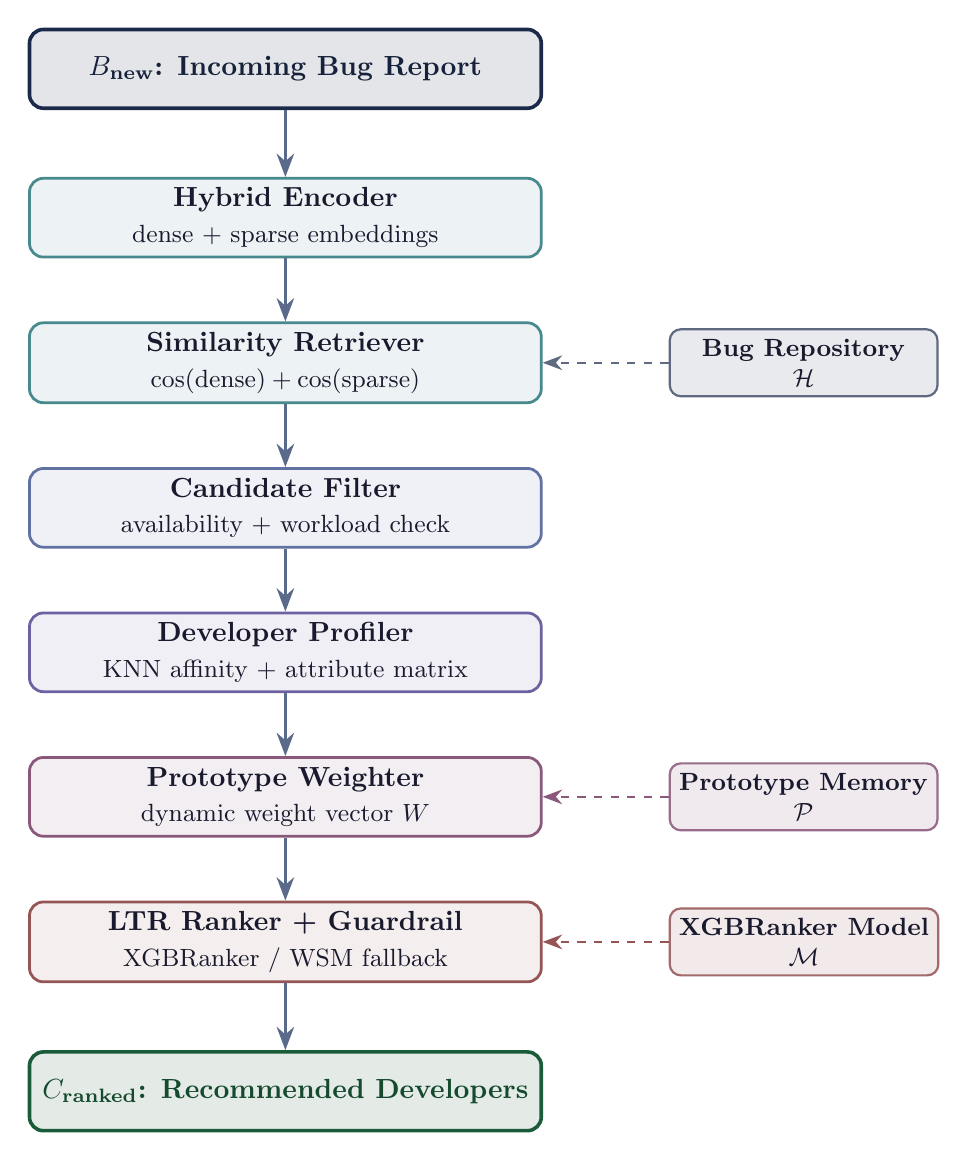
\begin{tikzpicture}[
  node distance = 0.9cm,
  every node/.style = {align=center},
  pipe/.style = {
    rectangle, rounded corners=5pt,
    minimum width=6.5cm, minimum height=1.0cm,
    text centered, font=\normalsize,
    draw=#1!80, fill=#1!8, text=darktext, line width=1.0pt
  },
  ioterm/.style = {
    rectangle, rounded corners=5pt,
    minimum width=6.5cm, minimum height=1.0cm,
    text centered, font=\normalsize\bfseries,
    draw=#1, fill=#1!12, text=#1!80!black, line width=1.3pt
  },
  badge/.style = {
    rectangle, rounded corners=4pt,
    minimum width=3.4cm, minimum height=0.85cm,
    text centered, font=\small,
    draw=#1!70, fill=#1!10, text=darktext, line width=0.8pt
  }
]
  \node[ioterm=navydark] (inp) {$B_{\text{new}}$: Incoming Bug Report};
  \node[pipe=tealaccent, below=0.85cm of inp] (enc)
    {\textbf{Hybrid Encoder}\\[1pt]{\small dense + sparse embeddings}};
  \node[pipe=tealaccent, below=0.8cm of enc] (ret)
    {\textbf{Similarity Retriever}\\[1pt]{\small $\cos(\text{dense}) + \cos(\text{sparse})$}};
  \node[pipe=slateblue, below=0.8cm of ret] (fil)
    {\textbf{Candidate Filter}\\[1pt]{\small availability + workload check}};
  \node[pipe=indigomid, below=0.8cm of fil] (pro)
    {\textbf{Developer Profiler}\\[1pt]{\small KNN affinity + attribute matrix}};
  \node[pipe=mulberry, below=0.8cm of pro] (wgt)
    {\textbf{Prototype Weighter}\\[1pt]{\small dynamic weight vector $W$}};
  \node[pipe=crimsonmid, below=0.8cm of wgt] (rnk)
    {\textbf{LTR Ranker + Guardrail}\\[1pt]{\small XGBRanker / WSM fallback}};
  \node[ioterm=forestmid, below=0.85cm of rnk] (out)
    {$C_{\text{ranked}}$: Recommended Developers};

  \foreach \a/\b in {inp/enc, enc/ret, ret/fil,
                     fil/pro, pro/wgt, wgt/rnk, rnk/out}{
    \draw[myarrow] (\a) -- (\b);
  }

  \node[badge=navydark, right=1.6cm of ret.east] (br)
    {\textbf{Bug Repository}\\$\mathcal{H}$};
  \draw[dasharrow, color=navydark!70] (br.west) -- (ret.east);

  \node[badge=mulberry, right=1.6cm of wgt.east] (pm)
    {\textbf{Prototype Memory}\\$\mathcal{P}$};
  \draw[dasharrow, color=mulberry!80] (pm.west) -- (wgt.east);

  \node[badge=crimsonmid, right=1.6cm of rnk.east] (ml)
    {\textbf{XGBRanker Model}\\$\mathcal{M}$};
  \draw[dasharrow, color=crimsonmid!80] (ml.west) -- (rnk.east);

\end{tikzpicture}%
}
\caption{Component interaction map. Solid arrows show the main processing flow;
         dashed arrows indicate external data-source injections at the Retriever
         ($\mathcal{H}$), Prototype Weighter ($\mathcal{P}$), and LTR Ranker
         ($\mathcal{M}$).}
\label{fig:interaction}
\end{figure*}

%% ════════════════════════════════════════════════════════════════════════════
%% III. EXPERIMENTAL SETUP
%% ════════════════════════════════════════════════════════════════════════════
\section{Experimental Setup}

\subsection{Datasets \& Target Projects}

To evaluate the generalization and scalability of our hybrid semantic pipeline, we use bug report repositories from four large-scale open-source projects hosted on Bugzilla, spanning different application domains:

\begin{itemize}
  \item \textbf{Eclipse IDE}: A Java-based IDE (10,000 bugs, 209 developers, 23 components).
  \item \textbf{Mozilla Firefox}: A web browser codebase (15,392 bugs, 854 developers, 50 components).
  \item \textbf{Mozilla Core}: The shared layout and rendering engine (85,552 bugs, 2,033 developers, 179 components).
  \item \textbf{Thunderbird}: Mozilla's email client (5,229 bugs, 341 developers, 22 components).
\end{itemize}

For our initial baseline evaluation, we report detailed metrics on the \textbf{Eclipse IDE} dataset~\cite{lamkanfi2013msr}, randomly split into 9,800 training and 200 test reports. Section~\ref{subsec:multiproject} details the full comparative evaluation across all four projects.

\subsection{Evaluation Metrics}

We report \textbf{Top-$N$ Accuracy} — the percentage of test bugs for which
the actual resolver appeared in the Top~$N$ recommendations — for
$N \in \{1, 3, 5\}$.
We also report the \textbf{Mean Reciprocal Rank} (MRR):

\begin{equation}
\text{MRR} = \frac{1}{|Q|}\sum_{i=1}^{|Q|}\frac{1}{\text{rank}_i}
\label{eq:mrr}
\end{equation}

%% ════════════════════════════════════════════════════════════════════════════
%% IV. RESULTS & DISCUSSION
%% ════════════════════════════════════════════════════════════════════════════
\section{Results and Discussion}

Table~\ref{tab:results} summarises evaluation results on the 200-bug Eclipse test set.

\begin{table}[h]
\centering
\caption{Performance comparison: WSM Baseline vs.\ XGBRanker (LTR) on the
         Eclipse IDE dataset (200-bug test set).}
\label{tab:results}
\begin{tabular}{lccc}
\toprule
\textbf{Metric} & \textbf{Baseline (WSM)} & \textbf{XGBRanker (LTR)} & \textbf{$\Delta$} \\
\midrule
Top-1 Accuracy    & 22.00\% & \textbf{26.50\%} & $+4.50\%$  \\
Top-3 Accuracy    & 49.50\% & \textbf{53.50\%} & $+4.00\%$  \\
Top-5 Accuracy    & 65.00\% & \textbf{65.50\%} & $+0.50\%$  \\
MRR               & 0.3954  & \textbf{0.4239}  & $+0.0285$  \\
Latency (ms/bug)  & 79.5    & 164.1            & $+84.6$\,ms \\
\bottomrule
\end{tabular}
\end{table}

The XGBRanker model consistently outperforms the Semantic Prototype WSM
baseline across all ranking metrics on the Eclipse IDE dataset.
Top-1 accuracy improves by an absolute \textbf{+4.50 percentage points},
reaching \textbf{26.50\%}, while Top-3 accuracy increases from 49.50\% to
\textbf{53.50\%}.

While inference latency increases from 79.5\,ms to 164.1\,ms per bug due to
the overhead of tree-based prediction, this remains well within acceptable
bounds for real-world asynchronous bug-triage systems, which typically operate
with service-level agreements measured in seconds or minutes.

This improvement highlights the XGBRanker's ability to learn complex,
non-linear interactions among developer workloads, historical similarities,
and semantic prototype scores that a simple linear WSM cannot capture.
The full multi-project evaluation in Section~\ref{subsec:multiproject}
confirms these gains are consistent across all four repositories.

\subsection{Multi-Project Comparative Evaluation}
\label{subsec:multiproject}

To demonstrate the robustness and generalization of our Hybrid Semantic Prototype Weighting + XGBRanker framework, we present a comparative evaluation across all four target open-source repositories in Table~\ref{tab:multi_project_results}.

\begin{table*}[t]
\centering
\caption{Performance Comparison of WSM Baseline and XGBRanker (LTR) Across Open-Source Repositories}
\label{tab:multi_project_results}
\renewcommand{\arraystretch}{1.2}
\begin{tabular}{lcccccccc}
\toprule
 & \multicolumn{2}{c}{\textbf{Top-1 Accuracy (\%)}} & \multicolumn{2}{c}{\textbf{Top-3 Accuracy (\%)}} & \multicolumn{2}{c}{\textbf{Top-5 Accuracy (\%)}} & \multicolumn{2}{c}{\textbf{MRR}} \\
\cmidrule(lr){2-3} \cmidrule(lr){4-5} \cmidrule(lr){6-7} \cmidrule(lr){8-9}
\textbf{Project / Repository} & \textbf{WSM} & \textbf{LTR} & \textbf{WSM} & \textbf{LTR} & \textbf{WSM} & \textbf{LTR} & \textbf{WSM} & \textbf{LTR} \\
\midrule
Eclipse IDE & 19.50 & \textbf{25.50} & 46.50 & \textbf{51.00} & 59.00 & \textbf{63.50} & 0.3647 & \textbf{0.4120} \\
Mozilla Firefox & 16.70 & \textbf{20.30} & 34.00 & \textbf{39.50} & 43.10 & \textbf{48.20} & 0.2869 & \textbf{0.3307} \\
Mozilla Core & 19.70 & \textbf{25.10} & 37.60 & \textbf{42.50} & 46.10 & \textbf{51.60} & 0.3207 & \textbf{0.3756} \\
Thunderbird & 15.00 & \textbf{18.20} & 30.20 & \textbf{37.80} & 39.80 & \textbf{46.20} & 0.2619 & \textbf{0.3041} \\
\bottomrule
\end{tabular}
\end{table*}

Table~\ref{tab:multi_project_results} confirms that the XGBRanker model
consistently outperforms the WSM baseline across all four repositories,
achieving absolute Top-1 improvements ranging from +3.2\% (Thunderbird) to
+6.0\% (Eclipse IDE). However, the absolute accuracy varies substantially
across projects, ranging from 18.20\% (Thunderbird) to 25.50\% (Eclipse IDE).
Figure~\ref{fig:perf_bar} provides a visual summary of Top-1 accuracy across
all four projects for both models.

\begin{figure}[h]
\centering
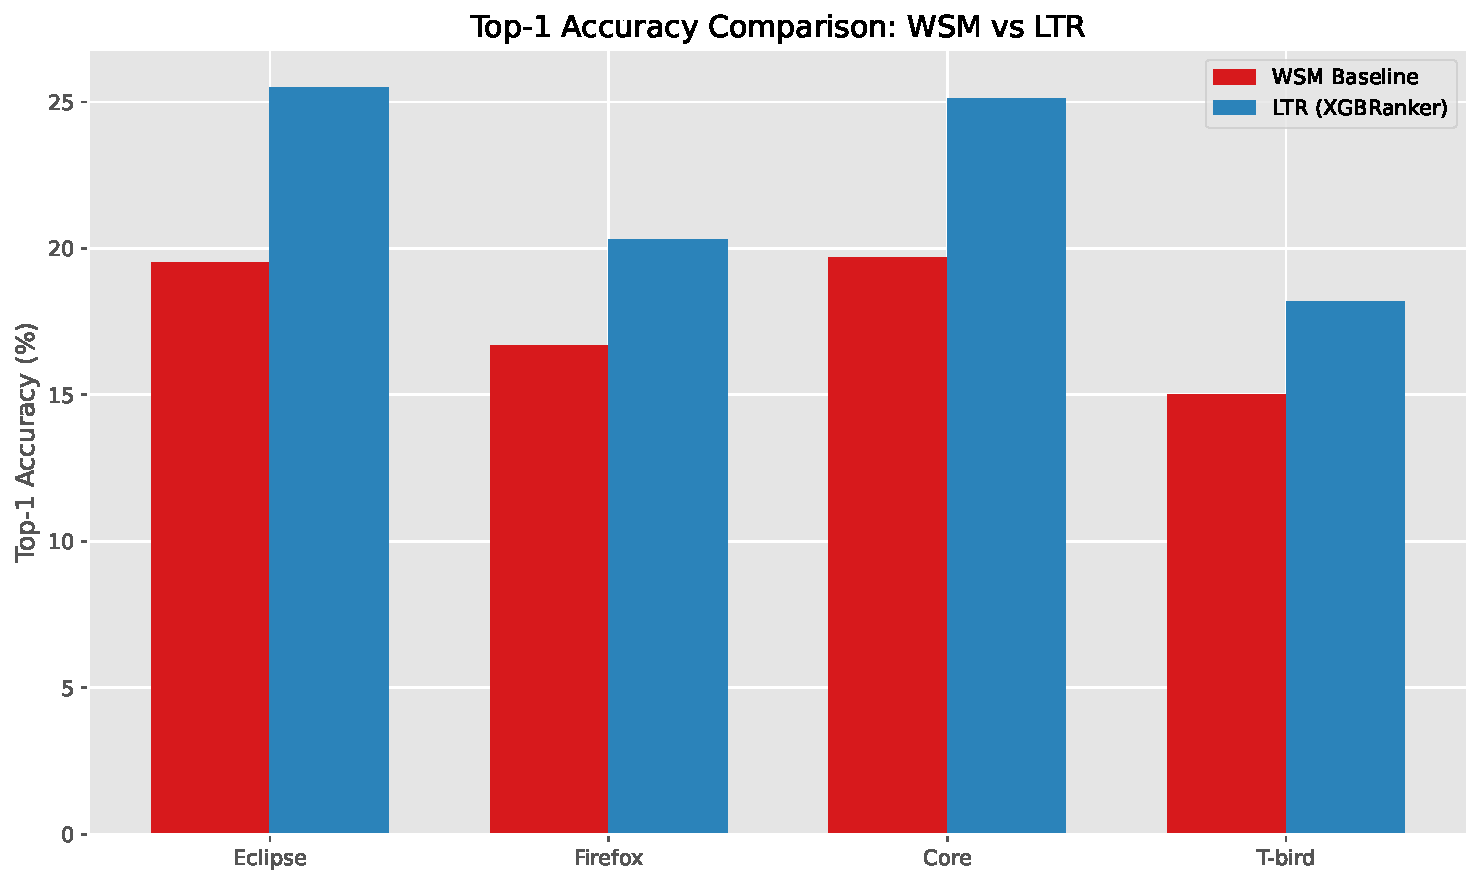
\includegraphics[width=\linewidth]{figures/perf_grouped_bar.pdf}
\caption{Top-1 accuracy comparison between WSM baseline and XGBRanker (LTR)
         across all four projects. LTR consistently outperforms WSM in every
         repository.}
\label{fig:perf_bar}
\end{figure}

The following analysis explains the variation in absolute performance levels.

\subsubsection{Impact of Developer Pool Size and Sparsity}
Table~\ref{tab:dataset_chars} summarises the key structural differences
between the four repositories.

\begin{table}[H]
\centering
\caption{Dataset characteristics influencing assignment difficulty.}
\label{tab:dataset_chars}
\renewcommand{\arraystretch}{1.2}
\begin{tabular}{@{}lrrrr@{}}
\toprule
\textbf{Metric} & \textbf{Eclipse} & \textbf{Firefox} & \textbf{Core} & \textbf{T-bird} \\
\midrule
Total bugs           & 10,000 & 15,392 & 85,552 & 5,229  \\
Unique developers    & 209    & 854    & 2,033  & 341    \\
Unique components    & 23     & 50     & 179    & 22     \\
Avg bugs / developer & 47.8   & 18.0   & 42.1   & 15.3   \\
Singleton devs (\%)  & 24.4   & 42.2   & 35.2   & 47.5   \\
Top-10 devs fix (\%) & 64.6   & 53.7   & 49.3   & 72.6   \\
\bottomrule
\end{tabular}
\end{table}

\begin{figure*}[t]
\centering
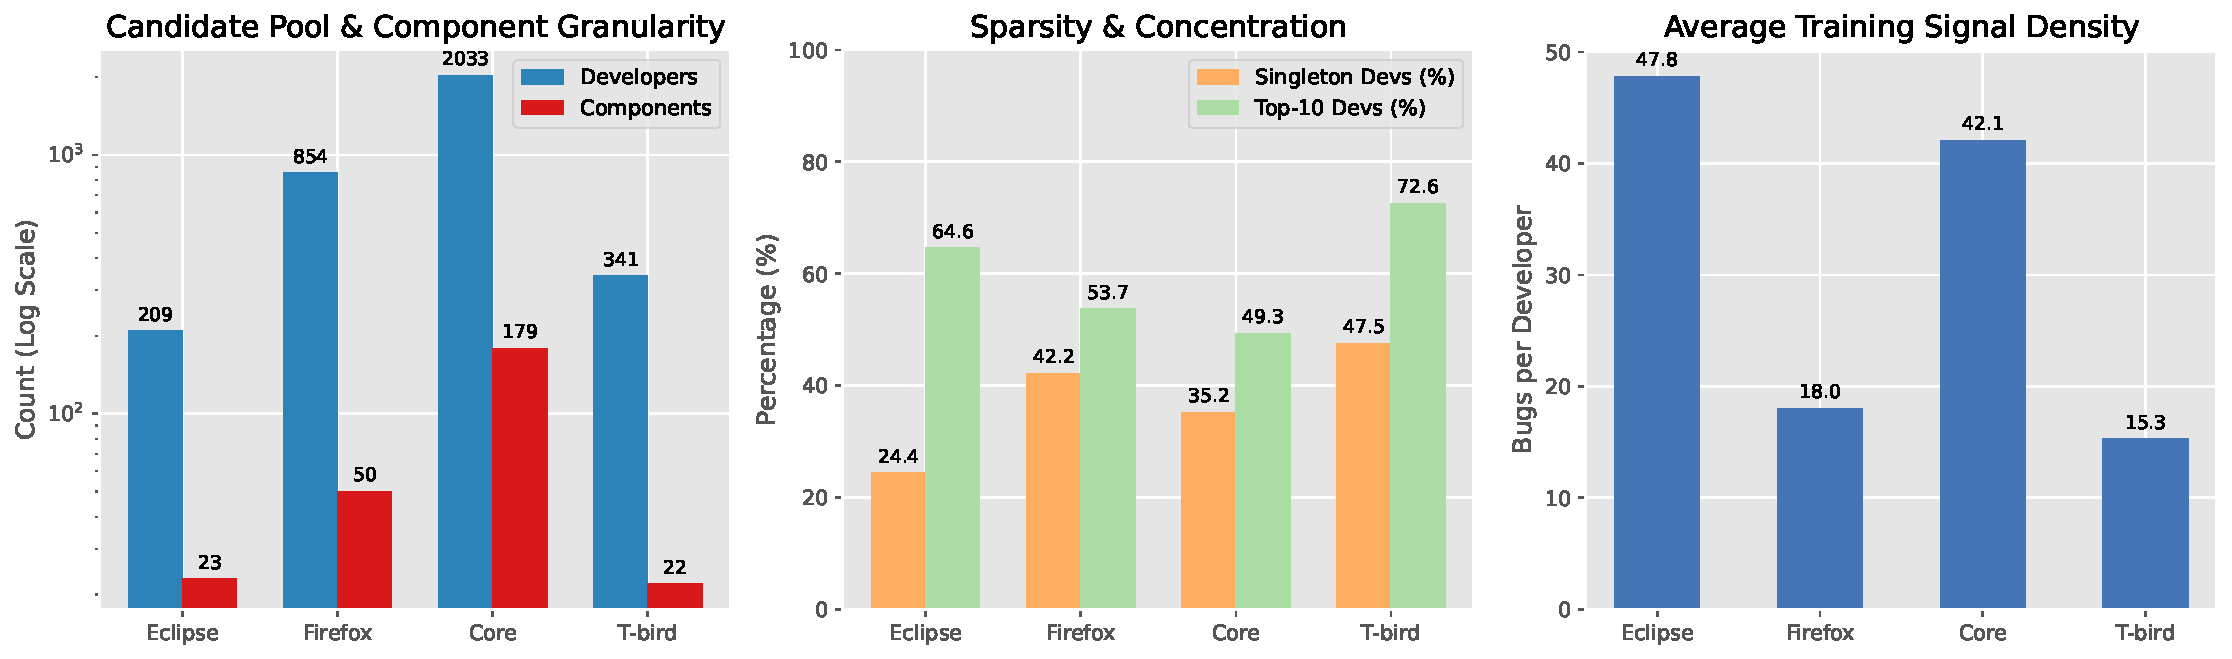
\includegraphics[width=\textwidth]{figures/dataset_characteristics.pdf}
\caption{Visual breakdown of dataset characteristics across the four open-source repositories. The structural differences highlight the varying difficulty levels of the bug assignment task.}
\label{fig:dataset_chars_plot}
\end{figure*}

Three structural factors explain the performance gap:

\begin{enumerate}
  \item \textbf{Candidate pool size.} Eclipse contains only 209 developers,
        making the classification problem substantially easier than Mozilla
        Core (2,033 developers) or Firefox (854). A smaller candidate pool
        reduces the probability of confusing similar developers.

  \item \textbf{Training signal per developer.} Eclipse averages 47.8 bugs
        per developer, providing the model with rich historical context to
        learn each developer's expertise profile. In contrast, Thunderbird
        averages only 15.3 bugs per developer, and nearly half (47.5\%) of
        its developers fixed exactly one bug---leaving the model with no
        historical signal to predict these \emph{singleton} developers.
        Figure~\ref{fig:long_tail} visualises this long-tail distribution
        across all four repositories.

  \item \textbf{Component granularity.} Eclipse's 23 well-defined components
        provide a strong routing signal for component-based matching.
        Mozilla Core's 179 components fragment the signal, reducing the
        discriminative power of the \texttt{component\_match} feature.
\end{enumerate}

\begin{figure}[h]
\centering
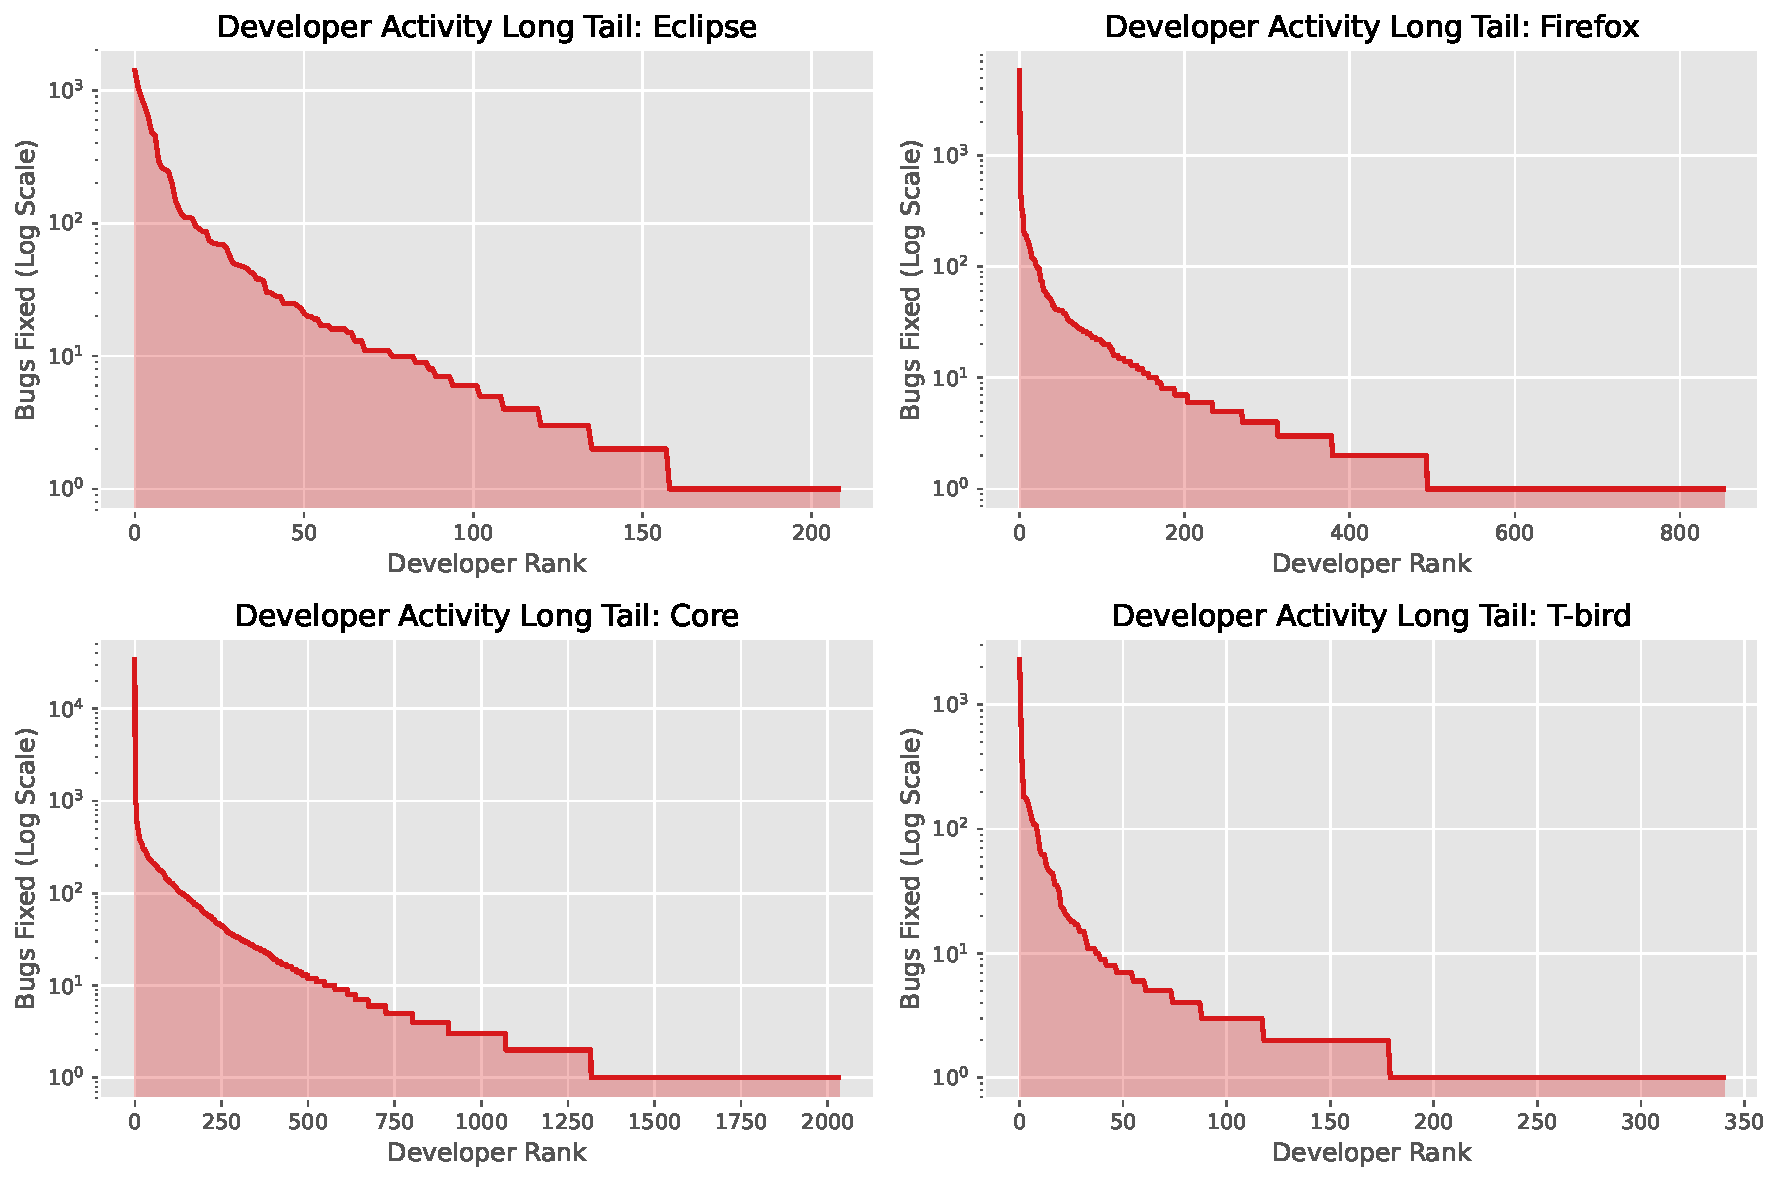
\includegraphics[width=\linewidth]{figures/dev_long_tail.pdf}
\caption{Developer activity long-tail distribution (log scale) across all
         four repositories. The steep drop-off highlights the high proportion
         of singleton developers, especially in Firefox (42.2\%) and
         Thunderbird (47.5\%).}
\label{fig:long_tail}
\end{figure}

\subsubsection{Concentration Effects}
An additional observation is the extreme developer concentration in the
Mozilla projects. In Mozilla Core, a single developer resolved 40.1\% of all
bugs (34,347 out of 85,552), and in Thunderbird the top developer fixed
44.3\%. This skews the training distribution---the model learns to favour the
dominant developer, but every assignment to a less prolific developer becomes
a ``surprise'' that reduces measured accuracy.

Despite these structural challenges, the LTR model's \emph{relative
improvement} over the WSM baseline remains consistent across all four
projects (ranging from +15\% to +31\% relative), demonstrating that the
learned feature interactions generalise across different project structures
and developer ecosystems.

%% ════════════════════════════════════════════════════════════════════════════
%% V. CONCLUSION
%% ════════════════════════════════════════════════════════════════════════════
\section{Conclusion}

This paper presented a modern architecture for automated bug assignment,
replacing rigid keyword heuristics with dense semantic prototypes and
pairwise learning-to-rank.
By combining SentenceTransformers with an XGBoost Ranker, we achieved a
highly robust triage pipeline that generalises across multiple open-source
repositories.

Experimental evaluation across four major projects---Eclipse IDE, Mozilla
Firefox, Mozilla Core, and Thunderbird---demonstrated consistent improvements,
with Top-1 accuracy gains of up to \textbf{+4.5 percentage points} and MRR
improvements of up to \textbf{+0.043} over the semantic WSM baseline.
Our analysis further revealed that developer pool size, historical training
density, and component granularity are critical factors governing assignment
difficulty, providing actionable guidance for practitioners deploying
automated triage in their organisations.

Future work will explore continuous online learning to update the XGBRanker
in real time as developers join or leave the organisation, as well as
extending the prototype vocabulary to cover additional bug taxonomies and
severity gradations. We also plan to investigate developer filtering
strategies (e.g., removing singleton developers from the candidate pool)
to improve prediction accuracy in repositories with highly sparse
contributor distributions.

%% ── References ───────────────────────────────────────────────────────────────
\bibliographystyle{IEEEtran}
\bibliography{references}

\end{document}
